\documentclass{mscLiterature}

% Zelf toegevoegd
\usepackage{todonotes}

\usepackage{pdflscape}
\usepackage{makecell}
\newcolumntype{M}[1]{>{\centering\arraybackslash}m{#1}}
\usepackage{tablefootnote}
%
%
% Thesis data
%\mscDepartment{Delft Center for Systems and Control (\textsmaller{DCSC})}%
\mscProgram{Systems and Control}
%Change if needed to
%\mscProgram{Mechanical Engineering}
\mscFaculty{Mechanical Engineering (ME)}%
\mscName{P.C.M. van Bentum}%
\mscDate{\today}%
\mscTitle{Optimizing small scale
district heating networks:
design and operation}%
\mscSubTitle{Cooltower use-case}%
\mscKeyWords{thesis, msc, subject}% only used in PDF properties
\mscCoverPicture{STYLESTUFF/COVER}% to place a picture ( here the example COVER.eps) on the back of the cover page
%
%
% Third party options (create text/logo on the copywrite page)
\mscThirdPartyText{The work in this thesis was supported by Eneco B.V. Their cooperation is hereby gratefully acknowledged.}
\mscThirdPartyLogo{figuresLIT/eneco_logo.jpg}
% NOTE: on the title page only the TU Delft logo is permitted.
%
%
%
% Finalize the thesis data
\setThesisInfo
%
% Use \includeonly{} to build only certain parts of your thesis
%\includeonly{introduction, real_chapter, empty_chapter, long_chapter}%
%
%PH Toegevoegd 24-10-2011
%allow (matlab) listing max 1pt flexibility between lines
\lstset{lineskip=0pt plus 1pt minus 0pt}
%
\begin{document}
%
%========================== Front matter ======================================
\frontmatter %
%
% Make the cover page and hell of a lot of title pages
\maketitle
%
%
% Abstract (does not appear in the Table of Contents)
\chapter*{Abstract}%

This is an abstract.


%
% table of contents, (\toc of \toclof of \tocloflot )
\toc
%
%
% %
% Preface
\chapter{Preface}

According to \textsc{WikipediA}, a preface (pronounced ``\emph{preffus}'') is an introduction to a book written by the author of the book. In this preface I can discuss the interesting story of how this thesis came into being. 

This is document is a part of my Master of Science graduation thesis. The idea of doing my thesis on this subject came after a discussion with my good friends Tweedledum and Tweedledee\ldots


% %
% Acknowledgements
\chapter{Acknowledgements}%

I would like to thank my supervisor \mscreaderone\ for his assistance during the writing of this thesis\ldots

By the way, it might make sense to combine the Preface and the Acknowledgements.  This is just a matter of taste, of course.

\vspace*{15mm}

Delft, University of Technology \hfill \mscname \\
\mscdate
% %
% Dedication page. 
\cleardoublepage
\thispagestyle{empty}
\vspace*{\stretch{1}}

% Put your own motto here, or dedicate your work to your Mom or whatever...
\begin{quote}
\noindent``In the future, airplanes will be flown by a dog and a pilot. And the dog's job will be to make sure that if the pilot tries to touch any of the buttons, the dog bites him.''
	
--- \emph{Scott Adams}
\end{quote}

\todo[inline]{moet mijn eigen quote in, of helemaal geen.}

\vspace{\stretch{3}}
\clearemptydoublepage
%
%========================== Main matter ======================================
\mainmatter
%
%
% Introduction
\chapter{Introduction} \label{chap::intro}
\section{Sustainable Heating}
The Paris Agreement, adopted in 2015, aims to limit global warming to well below 2$^{\circ}\text{C}$, and preferably to 1.5$^{\circ}\text{C}$ above pre-industrial levels. Achieving this goal requires significant decarbonization across all sectors, including heating. Within the European Union in 2023, around 62.5 \% of household energy consumption is used for space heating. However, only 23.5 \% of that energy currently comes from renewable sources \cite{EUenergie}. While in the Netherlands 82 \% of homes were still heated by individual gas boilers in 2021 \cite{NLenergie}.
This share of renewable sources must increase substantially if we are to meet the goals set by the Paris Agreement. District Heating Networks (DHN) are considered a key solution in the decarbonization of the heating sector, as they enable the integration of local renewable heat sources, renewable electricity, and waste heat \cite{KUNTUAROVA}.
% \todo[inline]{Here a story about the necessity of district heating networks for the problem of global warming. As a large part of the of the energy consumption of the Netherlands is heating. Where you can also mention the use for DHN in storing energy from the grid.} And then write about the fuel flexibility of district heating networks. And how big their part to play is in the future... afvalwarmte enzo, warmte opslag. Ook goed om kort het gebruik van individuele warmtepompen per huis te benoemen. 
% \todo[inline]{tip van Max: Hier kun je evt gebruik maken van het boek van Werner en Heat Roadmap Europe van Paardekoper et al.}

% The fundamental idea of district heating is sustainable as it wants to use local fuel or heat that would otherwise be wasted to meet the local heat demand \cite{bookMax}. Of course, this ideal is not always achieved and then it needs to make use of extra fuel but it shows the sustainable and effective mindset around district heating. 

\section{District Heating Networks}
Current district heating networks transport thermal energy by heated or cooled water through insulated pipes. These pipes are connected in an underground local network with one (or more) energy source(s), possibly storage, and buildings. The district heating (and cooling) networks facilitate the heating (and cooling) of these buildings. The temperature of the water flowing in and out of the building is called the supply and return temperature, respectively. There is a separate supply and return network with identical topology. 

District heating was commercially introduced in the late 19th century in the United States and at the beginning of the 20th century in Europe \cite{bookMax}. Currently, the use of district heating networks is increasing worldwide. The International Energy Agency predicts that 350 million housing units will be connected to a district heating network in 2030. Accounting for about 20 $\%$ of the global space heating needs \cite{IEAheating}. \\

In the first generation of district heating networks, heat was transported using steam, which led to too much corrosion due to condensation and high heat losses. Therefore, the second generation made use of pressurized water at 100 $^{\circ}\text{C}$, which still causes high heat losses \cite{FemkeJanssenLit}. Nowadays, the newest networks are of the fourth generation. These networks are implemented with a focus on decarbonization, in contrast to the previous three generations, which heavily relied on fossil fuels. The water temperature in these systems has a maximum of 60 - 70$^{\circ}\text{C}$. This was made possible by reducing heat loss of the buildings themselves and using floor heating, requiring a lower supply temperature \cite{FemkeJanssenLit}. This supply temperature lowers grid losses and makes it economically feasible to implement waste heat sources, such as excess heat from data centers. Also, heat pumps and solar collectors become more efficient, making it more suitable for implementing (seasonal) thermal energy storage. In the literature, a fifth generation of district heating networks is discussed. The extension of adding a cooling network is often mentioned in its definitions. However, the authors of the paper "\textit{Perspectives on fourth and fifth generation district heating}" conclude that it is a complementary technology, not a new generation of district heating networks \cite{4GDH5GDH}. 

\begin{figure}[h]
    \centering
    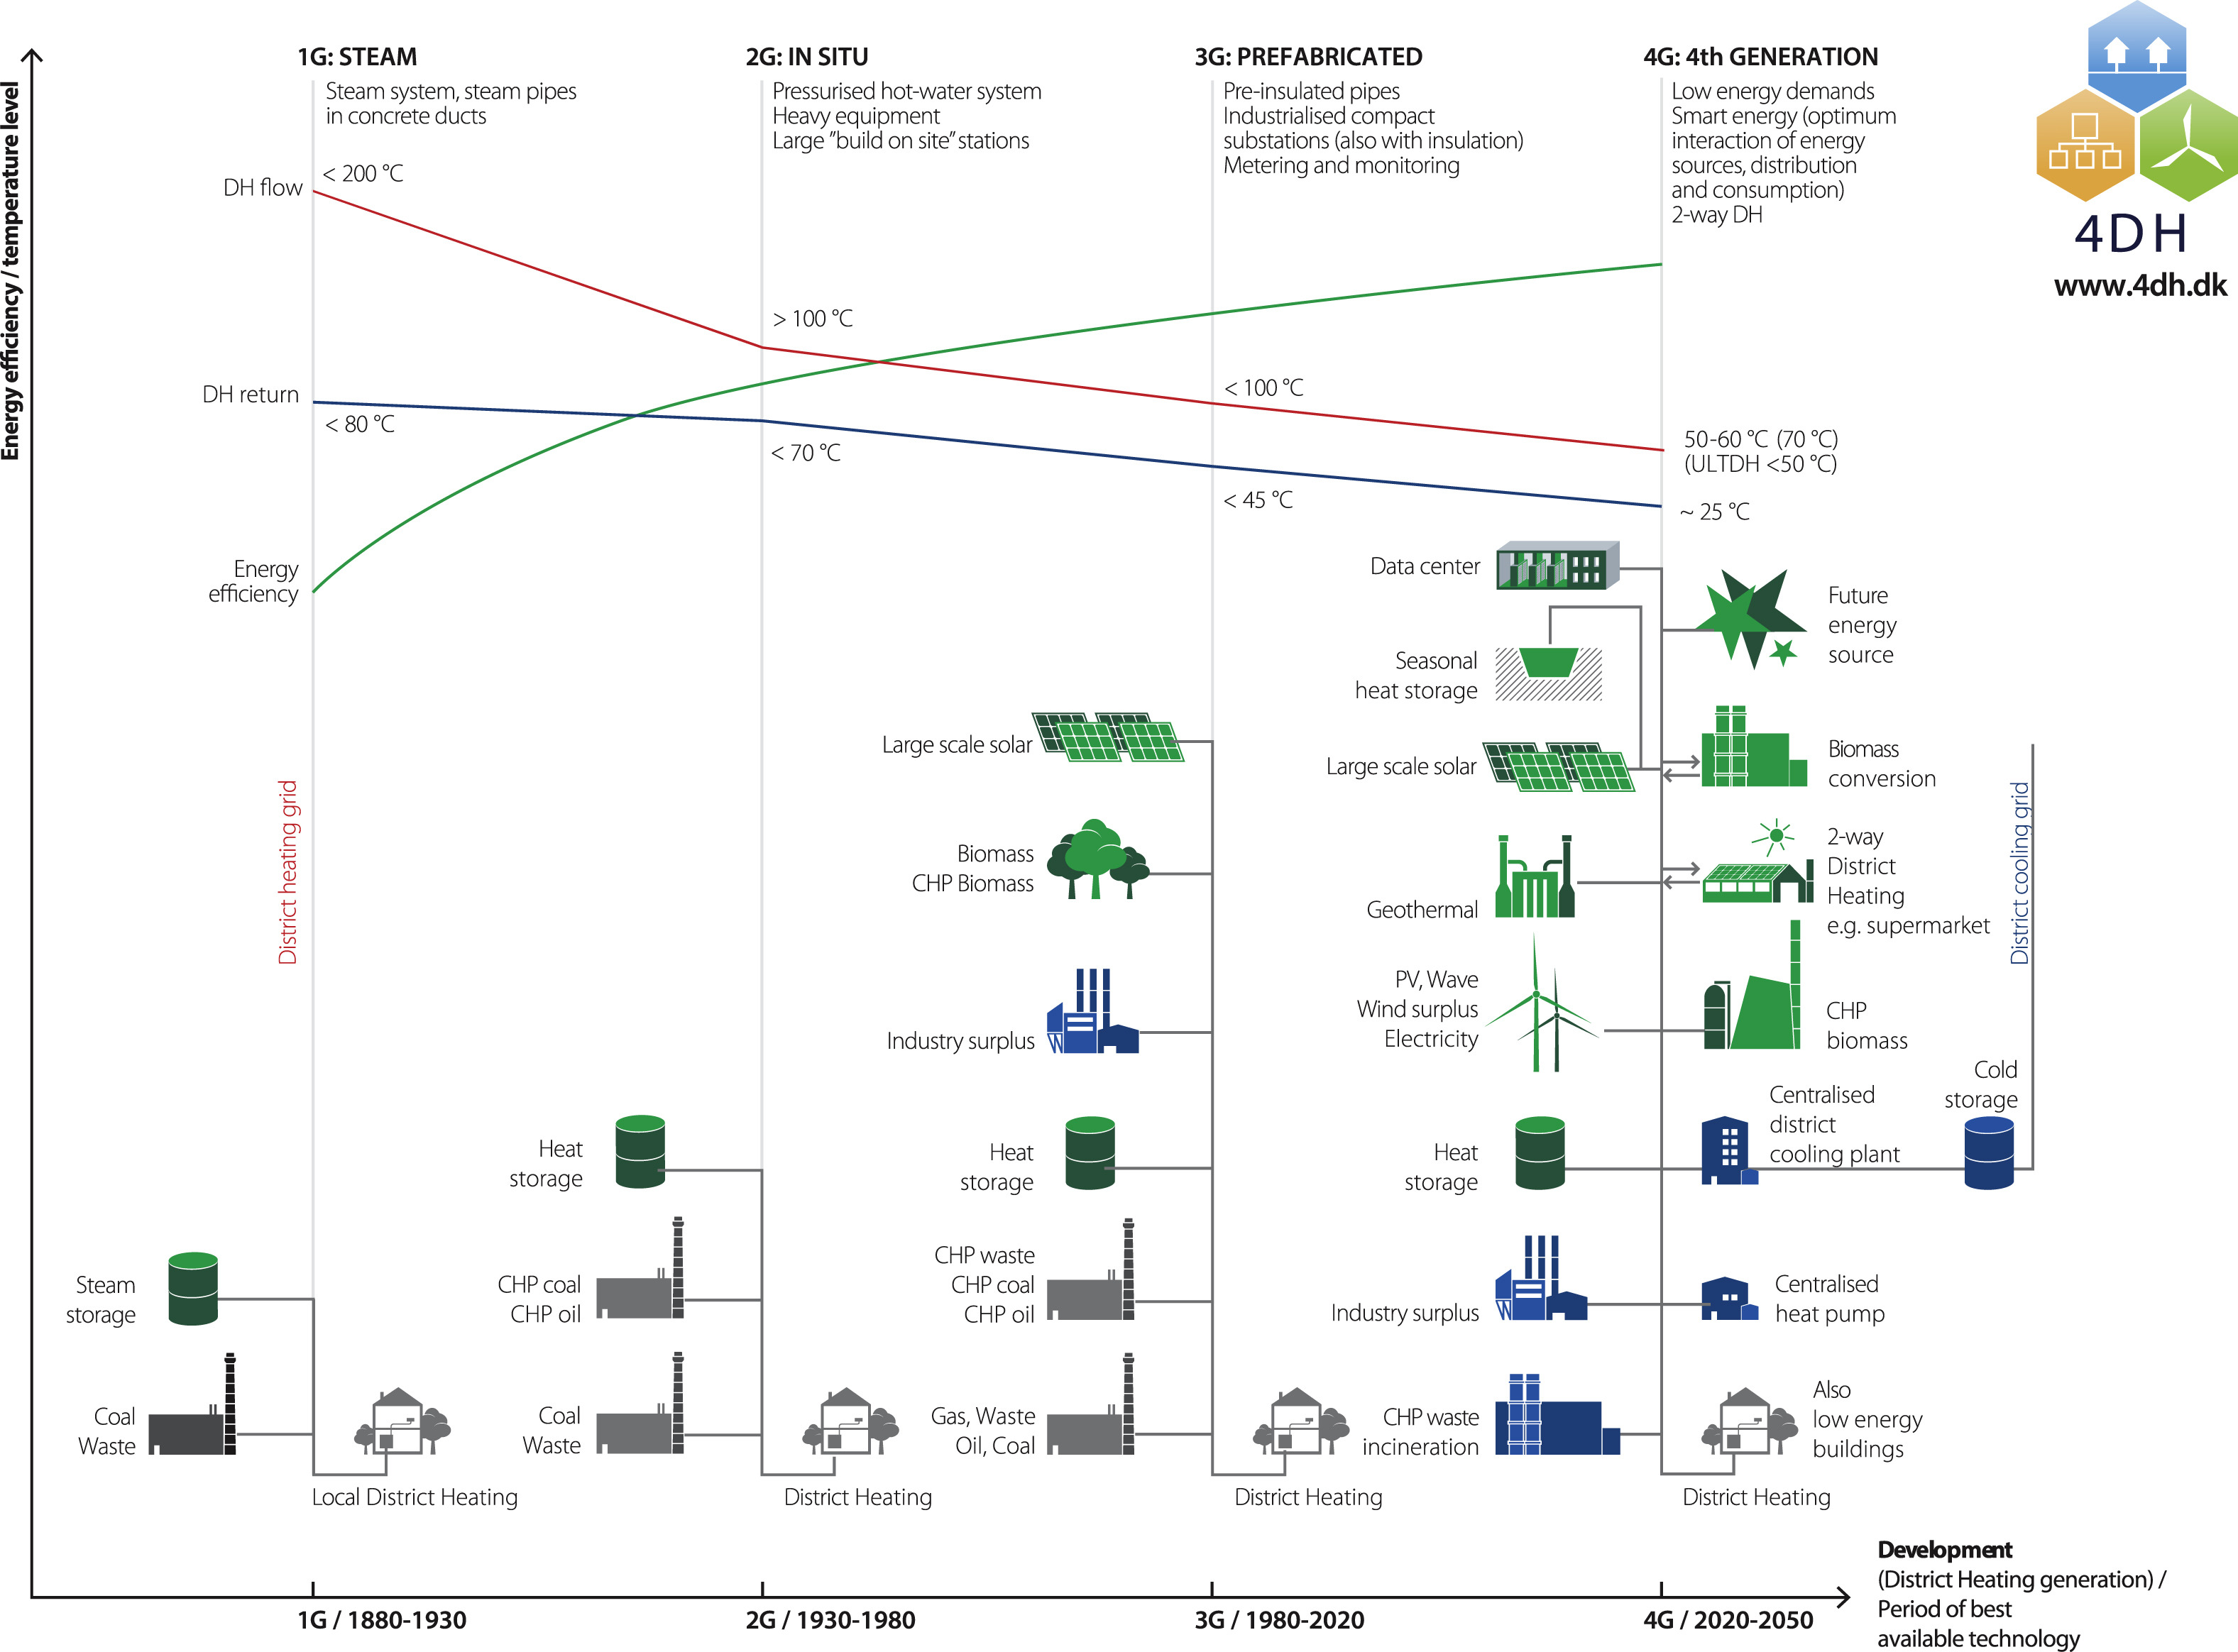
\includegraphics[width=\linewidth]{figuresLIT/GDH.jpg}
    \caption{The development of the district heating networks from the first up to the fourth generation \cite{4GDH5GDH}.}
    \label{fig:devDHN}
\end{figure}

\section{Changing Legislation}
In contrast to the electricity or gas networks, district heating networks are not connected to a national grid. This grid connects all producers and consumers and enables consumers to choose between energy providers. District heating networks are local networks connected to local heat producers. Narrowing the choice of energy providers. Most of the time, one energy provider owns and supplies the district heating networks, creating a monopoly. The Dutch government is working on new legislation, the "Collective Heat Act" (Wet Collectieve Warmte, Wcw), to change these monopolies and regulate these networks' heating and cooling prices. The government wants to stimulate the development of heating networks and guarantee their affordability, sustainability, and reliability. One of the provisions of the law states that collective heating networks serving 1,500 or more connections must be majority-owned for at least 51 $\%$ by public entities such as municipalities, provinces, or the national government \cite{WcWsite}. The Wcw allows more flexibility for heating networks with fewer than 1,500 connections. These smaller systems can be owned and operated by private entities, provided that they obtain an exemption from the municipality. The proposed law
must still be approved by both the House of Representatives (Tweede Kamer) and the Senate (Eerste Kamer) before it comes into effect. This legislative process may lead to changes to the bill and introduces uncertainty for energy companies.

\subsection{Decentralized Solutions}
Eneco is the market leader in District Heating in the Netherlands, with 150.000 customers. They have 68 heating networks, mainly in and around the cities of Utrecht, The Hague, Rotterdam, and Amsterdam. These networks differ in size, ranging from a couple of hundred to 59.000 connections \cite{warmtenetwerkenEneco}. The profitability of large networks already faced challenges due to their high investment costs. With the additional uncertainty caused by the Wcw, Eneco decided to focus on building smaller networks, called Decentralized Solutions (DCS) \cite{nos2025warmtenetten}. \\

% \begin{figure}
%     \centering
%     \includegraphics[width=0.5\linewidth]{}
%     \caption{Caption}
%     \label{fig:enter-label}
% \end{figure}
Decentralized Solutions are small local networks with up to 1,500 connections. These networks generate, store, and manage all their thermal energy near the consumer. They consist of consumers (households and larger users), one or more heat sources often including a heat pump, and heat and cold storage in the ground, and an underground pipeline network to connect them all. In some cases, the DCS is also connected to a larger nearby district heating system as a backup for the peak demand.

\begin{figure}[h]
    \centering
    \includegraphics[width=0.9\linewidth]{Literature Survey - DCSC template/figuresLIT/engelsDCSeneco.png}
    \caption{Depiction of Decentralized Solution. In this image, the DCS is not connected to a larger network for backup \cite{DCSeneco}.}
    \label{fig:DCS}
\end{figure}
The heat and cold underground storage is an Aquifer Thermal Energy Storage (ATES). The ATES generally consists of a heat pump and two wells. These wells are sandy layers underground where it simultaneously stores and extracts thermal energy by heating or cooling the groundwater. These are called hot or cold wells, respectively. The cold water used to cool the network is heated during the process and stored in the hot well. The same holds for the hot water that is stored in the cold well after being used for heating. When in summer the cold well is heated to above approximately 10 $^{\circ}\text{C}$, the heat pump is used as a backup cooling machine. In winter, the heat pump increases the temperature of the groundwater extracted from the hot well to 40 $^{\circ}\text{C}$ needed to heat the associated building. And during heating, the heat pump cools the used groundwater to 5-8 $^{\circ}\text{C}$ \cite{bloemendal2018hidden}. ATES addresses the seasonal mismatch between the availability and demand for heating and cooling in buildings. While it significantly reduces reliance on fossil fuels, the heat pump still requires a substantial amount of electricity to operate \cite{tudelft_ates_triplet}.

\subsection{Use case description}
During summer, the demand for heat decreases significantly, leading to increased return temperatures for the Decentralized Solutions. Return temperatures can reach up to 45-55 $^{\circ}\text{C}$, which is considered excessively high. Lowering the return temperature has certain benefits, which can be illustrated using the equation below. This relation shows how much thermal energy the water has lost (or gained) after it flows through the district heating network. 

\begin{equation}\label{eq::overallheat}
    \dot{Q} = \dot{m} c_p (T_s - T_r)
\end{equation}
$\dot{Q}$ [J/s] is the change in thermal energy of the water, $\dot{m}$ [kg/s] is the mass flow of the water, $c_p$ [J/(kg K)] is its specific heat capacity and $T_s$ and $T_r$ [K] are respectively the supply and return temperatures. 

If the supply temperature remains constant, the temperature difference will increase as the return temperature is reduced. This makes it possible to lower the flow rate of the water while still delivering the required heat. The pump will need less electricity, and the used pipes can be made smaller, saving on operational and initial costs. Also, the ATES heat pump will operate more efficiently because the required temperature drop for storing in the cold well is reduced.

One could also choose to lower the supply temperature, maintaining the initial temperature difference. This causes less heat loss as the supply temperature is closer to its surroundings. In addition, the network becomes more suitable for excess heat and renewable energy sources such as solar or geothermal energy, because these energy sources operate at temperatures lower than those of fossil fuels \cite{sustainableResources}. Besides the already mentioned increased efficiency of the ATES' heat pump when storing the water in the cold well, it becomes even better due to the reduced temperature lift required for heating the network. A too high return temperature might even lead to the malfunction and failure of a heat pump. Additionally, the solar collectors connected to the network become more efficient at a lower supply temperature \cite{booklowT}. Lowering supply temperature and flow rate can be performed simultaneously, however, this approach requires a strategic trade-off where one determines operational priorities such as cost minimization, decarbonization, or creation of flexibility. Moreover, reducing supply temperatures has its limits, as one must consider the minimal temperature constraints necessary for consumer demand satisfaction. Additionally, legislative reasons impact the minimum supply temperatures in the DHN. According to regulations, hot tap water must be kept at 55 degrees to prevent the growth of Legionella bacteria \cite{tapwaterWet}. 


This thesis aims to develop a dynamic simulation model of the Decentralized Solutions, to optimize their designs and operation in order to lower the return temperature, which is of major interest for Eneco. Since DCS networks can still differ from one another in terms of components and overall setup, it was decided to focus on a specific use case to make the scope of the research suitable for a MSc thesis. However, the model should be sufficiently generalizable such that it can be extended and scaled to other DCS networks.

The Cooltower was chosen for the use case. It is a 154-meter-tall flat in the city center of Rotterdam consisting of 272 apartments. It was completed in 2022 and was selected because it is the decentralized solution with the most sensors, providing the data for the eventual model validation.

\begin{figure}[h]
    \centering
    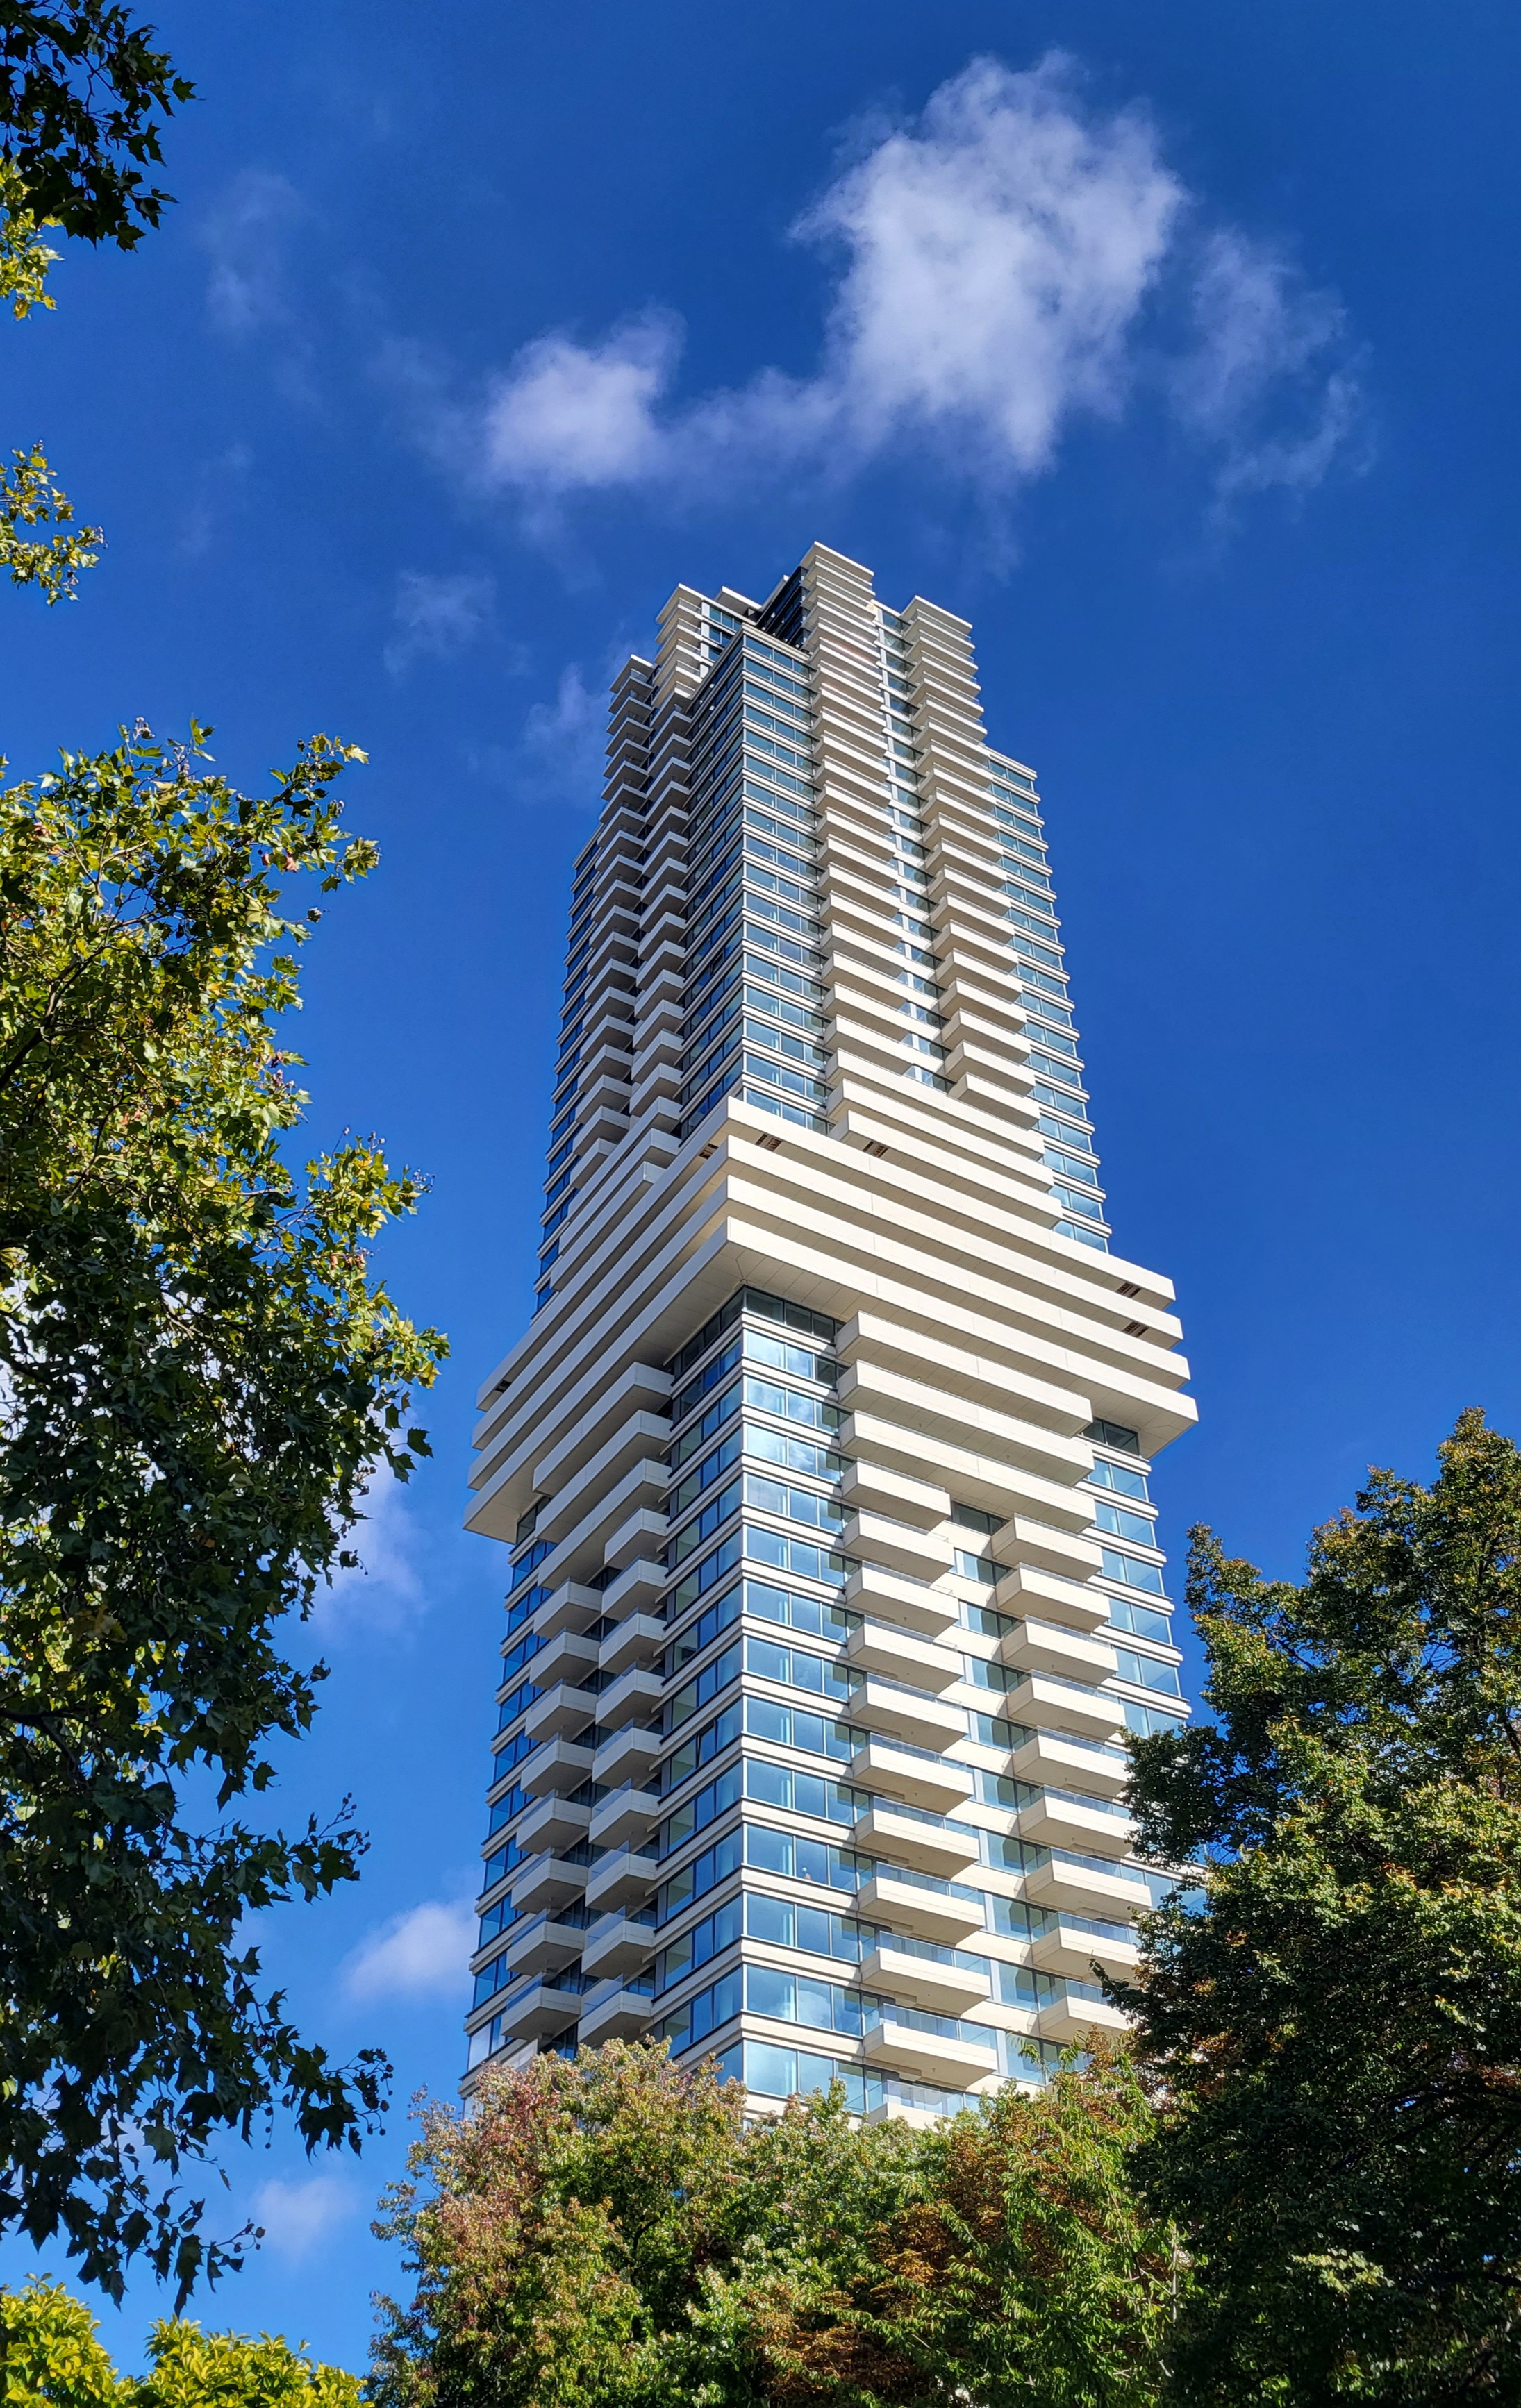
\includegraphics[width=0.5\linewidth]{figuresLIT/Cooltorenfoto.jpg}
    \caption{Picture of the Cooltower \cite{fotoCooltoren}.}
    \label{fig:Cooltoren}
\end{figure}

The Cooltower contains a heating and cooling network that is connected to an ATES below the building. Its network is also connected to the city heating network ('Stadsverwarming' in Dutch), which serves as a backup during peak demand. The building's internal heating and cooling network is split into lower and upper sections to prevent heat interface units (HIUs) on lower floors from experiencing excessive pressures. The scope of the thesis will remain on the district heating system within the Cooltower, with a focus on the thermodynamics and hydraulics of the heat distribution system within the building. If time permits, the dynamics of the ATES or the city heat network may be addressed at a later stage. Also the heat storage present in the system will not be taken into account as for now it is not being used.
This research looks at two actuators in the model to reduce the return temperature: the supply temperature and the overflow mechanism within the building. The overflow mechanism is a valve located at the top of the building where the supply pipeline directly flows into the return pipeline. To perform this optimization, the use of the data-driven method of Bayesian optimization will be investigated. The required accuracy of the simulation model introduces a computationally intensive optimization problem using this model. The thesis tries to overcome this problem by applying Bayesian Optimization.  

\newpage 
To conclude this section, the objective of this literature survey is formulated as follows.

{\centering
\textbf{Using the developed dynamic simulation model, we aim to investigate the possibilities to minimize return temperatures of the DCS by determining optimal control policies for the supply temperature and the overflow mechanism through data-driven Bayesian Optimization.}\par
}

The research must be done with the following model requirements in mind:
\begin{itemize}
    \item The discrete simulation timestep must be on the order of 1 minute. 
    \item The model should not only simulate the return temperature but also capture the internal hydraulic and thermodynamic behavior of the DCS heat distribution system.
    \item The model should be scalable and extendable, allowing it to be applied to other DCS networks.
    \item When the overflow mechanism turns out to be relatively simple and limits optimization performance, the optimization can additionally be performed by implementing a more advanced mechanism for the valve to evaluate its effects.
\end{itemize}

\section{Approach \& Outline}
First, Section \ref{chap::sysmodel} discusses methods for dynamically modeling the components of the heat distribution network of the Decentralized Solution in the Cooltower, including the modeling of heat demand and supply, and the development of a system framework. Next, Section \ref{chap::optimization} explores the optimization approaches used to reduce the return temperature, actuating the supply temperature, or an overflow mechanism. Finally, Section \ref{chap::PoA} presents a proposed plan for conducting the thesis.

% \begin{itemize}
%     \item Problem is too high return temperature in the summer
%     \item want bigger difference in temperature for heat pump, explain why.
%     \item also explain why they want 
%     \item dynamic model, while static models can already give some security concerns. 
%     \item Cooltower
%     \item has a DHN and DCN 
%     \item make difference between the high and low building
%     \item mention the overflow mechanism
%     \item name the components that will be modelled
%     \item clearly define the scope
% \end{itemize}


% This is a \LaTeX\ thesis and this is Chapter\ \ref{chap::intro}.

% \section{About \texorpdfstring{\LaTeX}{LaTeX}}

% \LaTeX\ is a document preparation system for the \TeX\ typesetting program. It offers programmable desktop publishing features and extensive facilities for automating most aspects of typesetting and desktop publishing, including numbering and cross-referencing, tables and figuresLIT, page layout, bibliographies, and much more.

% \LaTeX\ was originally written in 1984 by Leslie Lamport and has become the dominant method for using \TeX; few people write in plain \TeX\ anymore. The current version is \LaTeXe.

% If you want to know more about \LaTeX\ you better read \cite{texbook}.\index{LaTeX}


% \section{About Acronyms}

% This section contains an acronym of the \ac{DCSC}. The \ac{DCSC} is our department within the faculty of \ac{3mE} at \ac{TU}. \index{acronym}

% Acronyms are automatically listed in the Glossary in the back of this thesis. You have to define acronyms in \texttt{glossary.tex} using \verb"\acro{ACRONYM}{Full text}". You print an acronym by using the command \verb"\ac{...}". You can always force a full, long or short printout by using \verb"\acf{...}", \verb"\acl{...}" or \verb"\acs{...}" respectively.

% \begin{itemize}
%     \item \verb"\acf{DCSC}": \acf{DCSC};
%     \item \verb"\acl{DCSC}": \acl{DCSC};
%     \item \verb"\acs{DCSC}": \acs{DCSC}.
% \end{itemize}

% \section{About the Nomenclature}

% When you use symbols in your thesis -- as you probably will -- you can put them into the nomenclature listing (List of Symbols) at the back of your thesis. \tabref{tab:nomencl} shows the \LaTeX\ commands you need.\index{nomenclature}

% \begin{table}%
%     \centering
%     \caption{Nomenclature codes}
%     \label{tab:nomencl}
%     \begin{tabular}{llcl}
%         \toprule
%         Code & Usage & Example\\
%         \midrule
%         \verb"\gsymb{}" & Greek symbols & \gsymb{$\gamma$}{Path Angle}\\
%         \verb"\lsymb{}" & Letter symbols & \lsymb{$H(s)$}{Transfer function}\\
%         \verb"\supers{}" & Superscript symbols & \supers{max}{Maximum} &\emph{only printed in the List of Symbols} \\
%         \verb"\subs{}" & Subscript symbols & \subs{min}{Minimum} &\emph{only printed in the List of Symbols}\\
%         \verb"\others{}" & Other symbols & \others{[kts]}{Knots} \others{$^{\circ}$, [deg]}{Degrees} &\emph{only printed in the List of Symbols}\\
%         \bottomrule
%     \end{tabular}
% \end{table}

% \section{About {\textbackslash}(re)newcommand}
% As you will (soon) know the \LaTeX\ system makes use of commands in
% the form of \verb"\command". This can be used to make your life
% easier, since you can also define these commands yourself. Suppose
% that you often use an expression $e^{it}$. This would
% normally be written as \verb"$e^{it}$", or if already in math mode
% as \verb"e^{it}". Now you can define a command
% \verb"\eit" as follows\\
% \verb"\newcommand{\eit}{e^{it}}"\\
% This definition has to be placed in the so-called preamble, i.e.
% before the declaration\\ \verb"\begin{document}".\\ Now you can use
% this
% command in your text, so \verb"\eit" replaces \verb"e^{it}".\\
% Be aware that many commands are already in use by various packages.
% If you define an already existing command this will result in an
% error message. The best way to deal with this is to make sure your
% own command is unique, for instance by defining it as\\
% \verb"\newcommand{\MYeit}{e^{it}}".\\
% An alternative is to redefine the existing command by\\
% \verb"\renewcommand{\eit}{e^{it}}",\\
% but this is in general considered a tedious practice and should be
% avoided.
% See the \LaTeX\ documentation for more details and possibilities. You can also use arguments.\\
% %
% Don't underestimate the power of this feature. Suppose that you
% frequently use the expectation operator $E(x)$ in your text which is
% created with \verb"E(x)" (in math mode). Now your supervisor decides
% that he would prefer to see this as $\bf{E}(x)$. If you haven't
% defined your own command, you will have to go through the complete
% text, changing every instance. If you would have thought about it
% and
% would have defined originally\\
% \verb"\newcommand{\MyE{1}}{E(#1)}",\\
% using this in your text as \\
% \verb"\MyE{x}", \verb"\MyE{y}" etc.,\\
% then you can change this simply by adapting the definition to\\
% \verb"\newcommand{\MyE{1}}{\bf{E}(#1)}".

\chapter{System Modeling}\label{chap::sysmodel}
This section outlines the approaches to modeling the thermodynamic and hydraulic behavior of the Decentralized Solution in the Cooltower. It begins with an overview of the overall structure of the model. Subsequently, the hydraulic and thermodynamic modeling of the individual components is discussed. With particular attention given to the modeling of the valves. As unlike the other elements, the overflow mechanism (which is a valve) offers more flexibility within the optimization process, allowing exploration of alternative designs for further research. Afterwards, the peak and demand of the system are analyzed. Finally, a review of existing software tools for simulating district heating networks is presented. 

\section{Preliminaries}\label{sec::preliminaries}
Several general assumptions commonly used in the literature on  district heating networks and some dimesionless variables are outlined below. These assumptions are used throughout this chapter. Additional assumptions specific for particular methods are discussed in their dedicated sections.

This chapter focuses on modeling district heating networks. However, the same approach is applicable to district cooling systems, with modifications to account for the switch from heating to cooling.

\subsection{Modeling assumptions}
One of the most important modeling assumptions is that the hydraulic and thermodynamic systems can be assumed to be decoupled. This can be assumed as the speed of sound in the water is (1481 m/s at 20 $^{\circ}\text{C}$ \cite{speedofsound}) causing the changes in flow rate and pressure to be within seconds in a small district heating network like a DCS. In contrast with the spread of thermodynamic changes as these travel at the speed of the maximum flow rate, which is around 3 m/s. In combination with the assumptions that the water is incompressible, has a constant density and heat capacity, and that frictional heat is negligible, the two systems can be decoupled. 

Another important assumption based on the high speed of sound in water is that the hydraulics are assumed to be in steady-state. 

Furthermore, these are the other assumptions applied in this chapter. 
\begin{itemize}
    \item The fluid flow is turbulent and fully developed.
    \item The ambient temperature is constant along the length of the pipe.
    \item Homogeneous mixing at the pipe junctions.
    \item The pipes are cylindrical and are fully filled with water.
    \item No water leaves the pipe system.
\end{itemize}

% It is assumed that the hydraulics are in a steady state due to the high speed of sound in water (1481 m/s at 20 $^{\circ}\text{C}$ \cite{speedofsound}) causing the changes in flow rate and pressure to be within seconds in a small district heating network like a DCS. Whereas, the thermodynamic changes spread at a much lower speed with a maximum flow rate of around 3 m/s. Furthermore, it is assumed that the water is incompressible, has a constant density and heat capacity, and that frictional heat is negligible. Based on these assumptions, the hydraulic and thermodynamic systems can be assumed to be decoupled. In addition, it is assumed that the pipelines are cylindrical and completely filled with water. 
\todo{citaties naar waar de aannames ook gebruikt worden?}

% Andere aannames die mogelijk hier hier nog kunnen worden benoemd afhankelijk van hoe het gaat met de methods voor de pijpleiding:
% - zelfde diameter van de pijpleiding?
% - constant heat transmission coefficient
% - ambient temperature constant along the length of the pipeline
% - spatially homogenous velocity and temperature in the cross-seciton
% - heat diffusion in axial direction is neglected
% deze hierboven komen allemaal van Maurer.
% - turbulente flow? [Yvo Putter] -> Dit goed checken, moet ook turbulent flow aannemen voor de darcy weisbach
% - fully developed? [Yvo]
% - homogeneous mixing at pipe junctions
% - one directional flow?
\subsection{Dimensionless Numbers}
\textbf{The Reynolds Number (Re)} is the primary parameter correlating the viscous behavior of all Newtonian fluids \cite{white2011fluid}. It is a ratio between the internal and viscous forces within a fluid. And it is used as an indicator for a flow to be laminar or turbulent. 

\begin{equation}\label{eq::Re}
R e=\frac{\rho D v}{\mu}=\frac{4 \dot{m}}{\pi D \mu}
\end{equation}

Where $\rho$ [kg / m$^3$] is the density of the fluid, $v$ [m/s] the fluid velocity and $D$ [m] the diameter of the pipe, $\mu$ its dynamic viscosity [kg / (m $\cdot$ s] and $\dot{m}$ [kg/s] is the mass flow. 

\textbf{The Darcy friction factor (f)} can be found in the Darcy-Weisbach equation, which calculates the pressure flow drop through a pipe using the pipe flow. The coefficient can be determined using the Moody diagram, where $f$ is plotted against the Reynolds number for different relative roughnesses $\epsilon / d$. Or it can be determined analytically using the Colebrook-White equation \ref{eq:CoolbrookWhite}, which is the most popular method, for the transition region (2300 $\leq$ Re $\leq$ 4000) and the turbulent region (Re $\geq$ 4000) in smooth and rough pipes \cite{Darcyfrictionfactor}. This requires an iterative approach to determine $f$. There are also non-iterative methods, but they have a relative error to the Colebrook-White equation, however the authors of \cite{Darcyfrictionfactor} found that for certain correlations the error is negligible.

\begin{equation}\label{eq:CoolbrookWhite}
\frac{1}{\sqrt{f}}=-2 \log \left(\frac{\epsilon}{3.7 D}+\frac{2.51}{\operatorname{Re} \sqrt{f}}\right)
\end{equation}

With the roughness of the pipe $\epsilon$ [m].

\section{Model structure}
In \cite{GUELPA2016586}\cite{KECEBAS2012339}, a black box approach is applied, where the behavior of the entire DHN is put into one function, which is determined using data-driven methods. Another approach is to look at physical laws and parameters to create a model, the white box approach, which is the more conventional option used in the majority of the DHN modeling articles. The grey box model combines these two and can be found in \cite{grey1}\cite{grey2}. This literature survey focuses on the white box model.

District heating networks are branched or looped based networks, making them perfectly suited for modeling with a graph approach. The graph consists of nodes, which are junctions in the system, connected by edges. An edge is a pipe, potentially equipped with a heat exchanger, pump, or valve \cite{sibeijn2025economic}. On the edges, producers can add heat, and consumers can subtract it. The temperature at each node is determined by a weighted average of the incoming mass flows and their respective temperatures. All outgoing edges from the node are assigned the same temperature as the node itself. To calculate the mass flows and pressure within the network, Kirchhoff's two laws must be upheld. The first law asserts that the total mass flow entering and leaving a node must be equal, ensuring mass conservation. The second law requires that the net pressure drop around any closed loop in the network must be zero, maintaining pressure balance. The pressure loss within the pipes depends quadratically on the flow, making the hydraulics a system of non-linear equations. As we assume a decoupled system, the hydraulic problem is computed first, after which the obtained mass flow rates are used for the thermodynamic system. 

To solve this hydraulic system of non-linear equations, we assume that the demand and heat supply are known, leaving the pipe flows to be determined. This can be done by making use of iterative methods like Hardy-Cross \cite{HardyCross} and Newton-Raphson \cite{NewtonenHard}. These methods make an initial guess of the flow and then iteratively adjust this guess until it converges. Where the Hardy-Cross method runs through each loop independently, the Newton–Raphson method runs through all loops simultaneously \cite{NewtonenHard}. In \cite{STEVANOVIC}, the authors claim that they developed a method of square roots for solving the linearized system that outperforms the Hardy-Cross method in convergence time and validated it with real data. Also the aggregated models from \cite{LARSEN2002995} (also tested with real data) converge quicker (which is mainly interesting for big district heating networks) and overcome some of the limitations of the Hardy-Cross method.

The thermodynamic behavior of the edge in the system is described by a PDE. Different solutions for this equation are discussed in more detail in Section \ref{sec::thermo}

\section{Hydraulic modeling}
It is essential to know the pressure loss across all components, as this information, combined with Kirchhoff's laws, enables the determination of fluid flow throughout the district heating network. 

The total pressure loss of a pipe system can be divided into major and minor losses. The major pressure loss ($\Delta p_p$) is caused by friction along the length of the pipe and the height difference, the minor losses ($\Delta p_m$) are the result of the entrance or exit of the pipe, fittings, bends, valves, and sudden expansions and contractions of the pipes. Although they are called minor losses, a partially closed valve can cause a greater head loss than a long pipe \cite{white2011fluid}. Adding the heat exchangers ($\Delta p_{hex}$) to the major losses in this pipe system results in the following definition of total pressure change within a loop of the system. 

\begin{equation}
    \Delta p_{tot} = \sum \Delta p_{p} + \Delta p_m + \sum \Delta p_{hex} 
\end{equation}
The pressure loss over the pipes is discussed in Section \ref{sec::pipes}. Where $p_m$ depends on the type and size of the heat exchanger \cite{YvoPutter}, which needs to be determined for the DCS of the Cooltower. The minor losses are defined according to Equation \ref{eq::minorpres}.

\begin{equation}\label{eq::minorpres}
    \Delta p_m = \frac{\rho V^2}{2g} \sum \zeta
\end{equation}

The fluid velocity $V$ [m/s] and the loss coefficient $\zeta$ [-]. This formula holds that when all pipes have the same diameter, if the diameter changes, the fluid velocity will be affected. In that case, the losses need to be added separately. The manufacturer often provides the loss coefficients. However, the term is not based on the Reynolds Number or the roughness of the pipe, but solely on its diameter and assuming a turbulent flow \cite{white2011fluid}. If adding minor losses for a large pipe system becomes too cumbersome, one might choose to apply an additional percentage (5 to 20\%) on pipe friction losses \cite{echtephdthesis}. The pressure loss of the valves is discussed in more detail in Section \ref{sec::valves}.

%% ## HEAD
% In the literature, head (Equation \ref{eq::head}) is often used instead of pressure to describe hydraulic losses. 
% \begin{equation}\label{eq::head}
%     h = \frac{p}{\rho g}
% \end{equation}
% With head $h$ [m], pressure $p$ [Pa], gravitational constant $g$ [m/s$^2$], and the height to a certain reference point $z$ [m]. 

% The total head loss of a pipe system can be divided into major and minor losses. The major loss ($h_f$) is caused by the friction along the length of the pipe, the minor losses ($h_m$) are the result of the pipe entrance or exit, fittings, bends, expansions and contractions of the pipes and valves. Although they are called minor losses, a partially closed valve can cause a greater head loss than a long pipe \cite{white2011fluid}. Adding the heat exchangers ($h_{hex}$ to the major losses in this pipe system results in the following definition of the total head. 
% \begin{equation}
%     \Delta h_{tot} = h_f + \sum h_m + h_{hex} 
% \end{equation}
% The friction head loss $h_f$ is discussed in Section \ref{sec::pipes}. Where $h_m$ depends on the type and size of the heat exchanger \cite{YvoPutter}, which needs to be determined for the DCS of the Cooltower. The minor losses are defined according to Equation \ref{eq::minorhead}.

% \begin{equation}\label{eq::minorhead}
%     \sum h_m = \frac{V^2}{2g} \sum K
% \end{equation}

% The fluid velocity $V$ [m/s] and the loss coefficient $K$ [-]. This formula holds when all the pipes have the same diameter, as if the diameter changes, it affects the fluid velocity. In that case the losses need to be added separately. The loss coefficient is often provided by the manufacturer. However, the term is not based on the Reynolds Number or the roughness of the pipe, but solely on its diameter and assuming a turbulent flow \cite{white2011fluid}. The head loss of the valves is discussed in more detail in Section \ref{sec::valves} to further discover the modeling possibilities for the overflow mechanism. 


\subsection{Pipes}\label{sec::pipes}
An approximation of the 1-dimensional compressible Euler equations for cylindrical pipes is used to describe the dynamics within a pipe \cite{Krug2020}. The first two equations, the continuity equation and the 1D momentum equation, are needed for the calculation of the mass flows. They are stated down below.

\begin{equation}
\partial_t \rho+\partial_x\left(\rho v\right)=0
\end{equation}
\begin{equation}
\partial_t (\rho v)+\partial_x(\rho v^2)+ \partial_x p+\rho g \hat{z}  +f \frac{\rho}{2 D}|v| v=0
\end{equation}
Where $\rho$ [kg/m$^3$] is the water density, the water velocity $v$ [m/s], the pressure in the pipe $p$ [Pa], $g$ the gravitational acceleration [m/s$^2$], the slope of the pipe $\hat{z}$ [-], friction coefficient $f$ [-] and the diameter of the pipe $D$ [m]. According to the assumptions stated in Section \ref{sec::preliminaries} the following holds: $\partial_x v = 0, \partial_t \rho = 0$, $\partial_x \rho = 0$ and $\partial_t v = 0$. Making the continuity equation obsolete and results in the approximation of the momentum equation below \cite{sibeijn2025economic}. 
\begin{equation}\label{eq::mom}
\partial_x p + \rho g \hat{z} +f \frac{\rho}{2 D}\left|v\right| v=0
\end{equation}
Substituting $v = \frac{4 q}{\pi D^2}$ into \eqref{eq::mom} and discretizing $\partial_x p = \frac{\Delta p}{L}$ gives:
\begin{equation}
    \Delta p = p_{p} =  f \frac{8\rho L}{\pi^2 D^5}\left|\dot{m}\right| \dot{m} + \rho g L \hat{z}
\end{equation}
With the mass flow $\dot{m}$ [kg/m$^3$] and the length of the pipe $L$ [m]. The first term on the right side of the equation is equal to the Darcy-Weisbach equation, which describes the pressure loss due to the friction of the fluid with the pipe wall.  

%% ###HEAD
% Rewriting the equation into the head loss gives:

% \begin{equation}
%     h_f = f \frac{8 L}{\pi^2 d^5 g}\left|q\right| q + \hat{z}
% \end{equation}


\subsection{Valves}\label{sec::valves}
Valves regulate the pressure or flow in a pipe system. The Cooltower's heat distribution system contains multiple different types of valves. The pressure losses due to the valves can be calculated in a slightly different manner than the general relation for minor pressure loss in Equation \ref{eq::minorpres}, stated in Equation \ref{eq::realminorpres}, giving a more precise definition for the valves \cite{Artikelphdchris}. 

\begin{equation}\label{eq::realminorpres}
    \Delta p_{v} = \left( \frac{\dot{V}}{K_v} \right)^{2} \frac{\rho}{\rho_{ref}}    
\end{equation}
With the hydraulic conductivity parameter $K_v$  [m$^3$/h/$\sqrt{bar}$], the liquid flow $\dot{V}$ [m$^3$/h], the actual fluid density during the simulations $\rho$, and the fluid density during the manufacturer's $K_v$ measurements $\rho_{ref}$ (typically 1000 kg/m$^3$). The calculation of the valve characteristic $K_v$, which varies with the valve's opening position, depends on the valve type. It is important to mention that for small valve lifts, the $K_v$ value cannot be determined accurately because it exceeds the required tolerances of the basic shape of the valve. The valve's control range is determined up to a 10 percent deviation of the basic shape. When it goes outside of this control range, the valve becomes unpredictable. The manufacturer provides the control range \cite{echtephdthesis}.

\subsubsection{2-Way Control Valves}
At first, we have the 2-way control valves focused on controlling the flow. When this valve is a basic linear 2-way valve, $K_v$ can be determined using Equation \ref{eq::linear2valve}. Equation \ref{eq::equalpercentvalve} applies to an equal percentage valve. Both equations are in accordance with the VDI/VDE2173 standard \cite{VDI/VDE2713}. 

\begin{equation}\label{eq::linear2valve}
    \frac{K_v}{K_{vs}} = \left( 1 -\frac{K_{v,0}}{K_{vs}} \right) \frac{h_{lift}}{h_{\infty}} + \frac{K_{v,0}}{K_{vs}}
\end{equation}
\begin{equation}\label{eq::equalpercentvalve}
    \frac{K_v}{K_{vs}} = {\left(\frac{K_{vs}}{K_{v,0}} \right)}^{\frac{h_{lift}}{h_{\infty}} - 1}
\end{equation}

With the $K_v$ value for the completely opened value $K_{vs}$, the $K_v$ value at the points where the basic shape of the valve characteristic intersects with the y-axis $K_{v,0}$ and the dimensionless valve displacement $\frac{h_{lift}}{h_{\infty}}$ which ranges from 0 to 1 \cite{Artikelphdchris}. The differential pressure control valve is a specialized type of control valve designed to maintain a predefined pressure difference across a pipe. Unlike the previously discussed control valves, it directly controls the pressure drop over the pipe, not its flow. However, in practical applications, the valve is not ideal. The actual pressure difference across it may deviate from the setpoint. The modeling of such non-ideal behavior is further elaborated in \cite{echtephdthesis}.

\subsubsection{3-Way Control Valves}
There are also 3-way valves within the system. For these valves the hydraulic resistance is defined over two valve entrance ports A and B.
The valve characteristic pair can be complementary. In the case, it is a 3-way linear valve port A can be described using Equation \ref{eq::linear2valve} and port B using Equation \ref{eq::3way-valve}. Respectively, changing the valve characteristic formula into Equation \ref{eq::equalpercentvalve} results in a 3-way equal percentage valve. However, sometimes the ports contain two different valve characteristics. 

\begin{equation}\label{eq::3way-valve}
    \frac{K_{v,B}}{K_{vs}} = 1 - \frac{K_{v,A}}{K_{vs}}
\end{equation}

The heat interface units present in the Cooltower, the Arctic WKW-S 4P \cite{fortes_wkw_s_4p}, contain a 6-way ball valve. This valve can be modeled as two interconnected 3-way valves with synchronized control logic. In this simplified model, each valve operates in a binary manner, either fully open or fully closed. Together, they determine whether the heat interface unit is in heating or cooling mode. Sometimes, the 6-way valve can also perform flow control, but not in our case.

\subsubsection{Overflow Mechanism}
\todo[inline]{Kan hier mogelijk nog wat zeggen over de square opening valve}
\todo[inline]{find out what type of valve is really in the system.}

Other more common valves present in hydraulic systems are 

Modulating valve [DHN bijbel p 371]
(three port) control valve -> the control valves 
thermostatic radiator valves
throttling valves

\subsection{Pumps}
Pumps supply the pressure necessary for the fluid to flow through the network. Centrifugal pumps are the most
commonly used pumps in district heating networks. The pump can be described by the pump characteristic, in which the pump pressure or head is plotted against the flow rate. The plot is for multiple rotation pump rotation speeds. The system head curve is also plotted, the system operation points are where both curves intersect. 
\begin{figure}
    \centering
    \includegraphics[width=0.5\linewidth]{}
    \caption{Caption}
    \label{fig:enter-label}
\end{figure}

\section{Thermo-Dynamic modeling}\label{sec::thermo}
\subsubsection{Node Method}
\subsubsection{Lagrangian approach}
\subsubsection{other methods for pipes}
\subsection{Thermal conductivity}
It is assumed that the fluid velocity is high enough to neglect heat conduction in the direction of the flow. Therefore only the heat convection of the fluids needs to be taken into account as well as the heat conduction of the plate material. Uo is the overall heat transfer coefficient between the two fluids. This heat transfer coefficient is the reciprocal of the overall heat transfer resistance (3-13). 
\todo[inline]{van de literatuur studies Femke Jansen}
\subsection{Heat Exchanger}
LMTD, NTU
over nadenken hoe je dit dan doet voor zo'n afleverset
\subsection{Other components}

\section{Head supply}
CHP en ATES

\section{Head demand}


\section{Simulation Software}
- tabel voor alle mogelijke simulatie software die gebruiken van word
- daarin verwijzen welke technologie ze gebruiken
- cfd programmas ook naar gekeken maar te uitgebreid. 


\chapter{Optimization}\label{chap::optimization}
\todo[inline]{eerst een stukje over algemen optimalisatie}
\todo[inline]{Hier kijken naar optimalisatie manieren met valves}
\todo[inline]{Valve actuator, pagina 54 phd thesis}
\todo[inline]{Valve authority, kijk op pagina 111 van phd thesis}
\todo[inline]{Dynamic pressure control valve}
\todo[inline]{Bayesian optimisation}
\include{Conclusion}
%
%
%========================== Appendices =======================================
\appendix
%
% %
% An Appendix
\chapter{The Back of the Thesis}

% Appendices are found in the back. 


% \section{An Appendix Section}

% \subsection{An appendix subsection with C++ Listing}

% \lstset{language=C++}
% \lstinputlisting{test.c}

% \subsection{A MATLAB listing}

% \lstset{language=matlab}
% \lstinputlisting{test.m}

% %
% Another appendix chapter
\chapter{Yet Another Appendix}


\section{Test Section (Again?)}

Ok, all is well.


%========================== Back matter ======================================
\backmatter
%
% Bibliography
\bibliographystyle{unsrturl} % or upload this style file
\bibliography{MyBib} % without the .bib extension
%
%
% Glossary
\chapter{Glossary} %
%
% \printacronyms
% \begin{acronym}[\hspace{0.8in}] % 0.8in is also used by the nomenclature
% 	\acro{3mE}[3\textlarger{m}E]{Mechanical, Maritime and Materials Engineering}%
% 	\acro{AMS}{American Mathematical Society}%
% 	\acro{DCSC}{Delft Center for Systems and Control}%
% 	\acro{TU}[TU D\textlarger{elft}]{Delft University of Technology}%
% \end{acronym}%
% %
% %
% % Nomenclature
% \printnomencl%
%
% Index
\cleardoublepage
\printindex

\end{document}
